%*****************************************
\chapter{Grundlagen}\label{ch:preliminaries}
%*****************************************

Dieses Kapitel wird nun zunächst die theoretischen Grundlagen betrachten, die zum Verständnis und zur Durchführung der geplanten methodischen Vorgehensweise notwendig sind.
Somit bekommen Fachfremde einen Einblick in die Themenbereiche der medizinischen Informatik und des Semantic Webs.

\section{Medizinische Informatik}\label{sec:mi}

Die Medizinische Informatik beschäftigt sich mit der systematischen Gewinnung, Verarbeitung, Speicherung und Bereitstellung von Daten im gesamten Gesundheitssystem. 
Die \ac{GMDS} beschreibt die Medizinische Informatik folgendermaßen: \\

\begin{addmargin}[10pt]{10pt}
\enquote{Die Medizinische Informatik ist die Wissenschaft der systematischen Erschließung, Verwaltung, Aufbewahrung, Verarbeitung und Bereitstellung von Daten, Informationen und 	Wissen in der Medizin und im Gesundheitswesen.} \\
\end{addmargin}

Das wichtigste Ziel der medizinischen Informatik ist, die richtigen Informationen zur rechten Zeit am richtigen Ort in der richtigen Form dem richtigen Adressaten zur Verfügung zu stellen, um eine qualitative und effiziente Patientenversorgung sicherzustellen. \citep[vgl.]{winter_health_2011}

\subsection{Daten, Information, Wissen}

Die Begriffe Daten, Information und Wissen stehen in einer hierarchischen Beziehung zueinander.

\textbf{Daten} sind Symbole und Zeichen. Sie sind die Grundlage für Kommunikation, Interpretation und Verarbeitung von Menschen oder Maschinen.

\textbf{Informationen} sind in einem semantischen Kontext gesetzte Daten.
Informationen stellen Kenntnisse über Sachverhalte oder Personen dar.

\textbf{Wissen} beschreibt somit die gesammelte Information, die über die Begriffe einer bestimmten Domäne zur Verfügung stehen. 
Die Kenntnisse über diesen Sachverhalt ermöglichen es, fundierte Entscheidungen zu treffen und Probleme zu lösen.

\subsection{Krankenhausinformationssysteme}

Bevor man den Begriff Krankenhausinformationssystem definieren kann, werden erstmal die Begriffe System und Informationssystem betrachtet. \newline

Ein \textbf{System} ist eine Menge von Personen, Gegenstände, Ereignisse und deren Beziehungen zueinander. 
Ein System kann aus mehreren Subsystemen bestehen, die wiederum ein System darstellen. \citep[vgl.]{winter_health_2011} \newline

Ein \textbf{Informationssystem} ist der Teil einer Institution, das sich mit der Verwaltung und Speicherung von Daten, Informationen und Wissen beschäftigt.
Ein Informationssystem umfasst sowohl die gesamte Informationsverarbeitung als auch die dazugehörenden menschlichen oder technischen Akteure. \citep[vgl.]{winter_health_2011} \newline

Demnach ist Krankenhausinfromationssystem wie folgt definiert: 

\begin{definition}
	\enquote{Ein Krankenhausinformationssystem ist das sozio-technische Subsystem eines Krankenhauses, das die gesamte Informationsverarbeitung sowie die zugehörigen menschlichen oder technischen Akteure in ihren jeweiligen Informationsverarbeitungsrollen umfasst.} \citep{winter_health_2011}
\end{definition}

\subsection{Informationsmanagement in Krankenhäusern}

Betrachtet wird erstmal das Informationsmanagement allgemein, bevor das Informationsmanagement in Krankenhäusern erläutert wird.
\citet{gehring2022informationsmanagement} beschreiben das Informationsmanagement wie folgt: \\

\begin{addmargin}[10pt]{10pt}
\enquote{Das Informationsmanagement ist eine Führungsaufgabe, die darauf abzielt, die Nutzung der Ressource Information, die Verarbeitung und Bereitstellung von Informationen
mittels Anwendungssystemen sowie zum Systembetrieb eingesetzte IT-Infrastruktur so zu
organisieren, dass unter Ausschöpfung des strategischen Potenzials von IuK-Technologien
ein möglichst hoher Beitrag zum Unternehmenserfolg erwirtschaftet wird.} \\
\end{addmargin} 

Demnach ist das Informationsmanagement in Krankenhäusern das Management des Krankenhausinformationssystems.
Die Aufgaben im Rahmen des Informationsmanagements in Krankenhäusern sind die Folgenden:

\begin{itemize}
\item die Planung des Krankenhausinformationssystems und seiner Architektur
\item die Steuerung der Einrichtung und des Betriebs des \ac{KIS}
\item Überwachung der Entwicklung und des Betriebs des \ac{KIS} im Hinblick auf die strategischen Ziele des Krankenhauses \citep[vgl.]{winter_health_2011}
\end{itemize}

\section{Semantic Web}\label{sec:sw}

Das Semantic Web ist ein Netz von Daten, die so beschrieben und verknüpft sind, dass ein Kontext oder eine Semantik entsteht, die sich an definierte Grammatik- und Sprachkonstrukte halten. \citep[vgl.]{hebeler_semantic_2009}
Der Technologie-Stack worauf das Semantic Web basiert, wird in der Abbildung \ref{fig:abb1} dargestellt.
Die Abbildung zeigt einerseits die logische Struktur des Semantic Webs, im Bild die Concepts\&Abstractions Seite des Technologie-Stacks und die andere Seite zeigt die eingeführten Technologien.
Das ist die Specifications\&Solutions Seite des Würfels.
In diesem Unterkapitel werden die grundlegenden Technologien des Semantic Webs vorgestellt, die relevant für die vorliegende Arbeit sind.

\begin{figure}[h]
	\centering
    	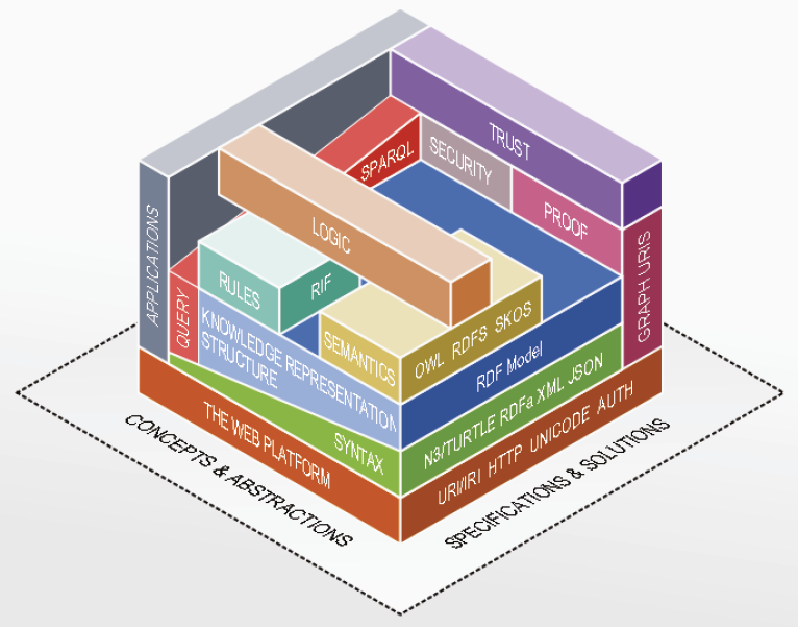
\includegraphics[width=0.85\textwidth]{Images/Linked_Data_Tech_Stack}
	\caption{Semantic Web Technologie Stack}
   	\caption*{\small Quelle: \url{https://smiy.files.wordpress.com/2011/01/sw_layercake.png}}
   	\label{fig:abb1}
\end{figure}

\subsection{World Wide Web}

Das \ac{WWW} ist eine Initiative, die verfügbare Technologien nutzt, um ein globales Informationsuniversum zu schaffen.
Grundlegend besteht das \ac{WWW} aus Inhalten, die primär an Menschen ausgerichtet sind.
Das \ac{WWW} besteht aus einer Vielzahl an Websites, die durch Hyperlink miteinander vernetzt sind.
Im Gegensatz zum Semantic Web ist die Semantik des \ac{WWW} nicht ersichtlich.
Man wird von einer Seite zur anderen mittels \ac{URL}s weitergeleitet und der Nutzer muss in der Regel die Semantik selber ableiten.
Inhalte im \ac{WWW} werden beispielsweise mit Hilfe von HTML, CSS oder JavaScript formatiert. \citep[vgl.]{hebeler_semantic_2009}

Das Semantic Web soll als eine Erweiterung des WWW betrachtet werden.
Die Tabelle \ref{table:1} vergleicht die Eigenschaften des \ac{WWW} und des Semantic Webs.

\begin{table}[ht]
\begin{tabulary}{\textwidth}{LLL}
\toprule
Feature & WWW& Semantic Web \\
\midrule
grundlegende Komponente & unstrukturierte Inhalte & formale Statements \\ 
primäre Zielgruppe & Menschen & Applikationen \\ 
Links & geben den Ort an & geben den Ort und die Bedeutung an \\ 
vorwiegendes Vokabular & Formatierungsanweisungen & Semantik und Logik \\ 
Logik & informell/nicht standardisiert & Beschreibungslogik \\ 
\bottomrule
\end{tabulary}
\caption{Vergleich zwischen WWW und Semantic Web.}
	\caption*{\small Quelle: \cite{hebeler_semantic_2009}}
\label{table:1}
\end{table}

\subsection{Ontologien}

Ontologien sind eine Form des Wissensmanagements und bilden den Kern aller Semantic Web Applikationen. 
Sie werden eingesetzt, um Wissen in einer strukturierten Weise zu organisieren.
Die Definition, die am häufigsten in der Literatur vorkommt, ist von \citet{gruber_translation_1993}:

\begin{definition}
  Eine Ontologie ist eine explizite Spezifikation einer Konzeptualisierung(Begriffsbildung).
\end{definition}

\noindent Aus Grubers Perspektive repräsentiert eine Ontologie das Wissen einer bestimmten Domain, wobei Objekte und deren Beziehungen mit Hilfe eines Vokabulars beschrieben werden. \citep[vgl.]{breitman_semantic_2007}

Im Bereich des Semantic Webs werden Ontologien als Graphen oder Netzwerkstrukturen betrachtet, die aus den folgenden Elementen bestehen:

\begin{itemize}
	\item eine Sammlung von Objekten (die Knoten des Graphs)
	\item eine Sammlung von Beziehungen, die die Objekte miteinander verknüpfen (Kanten des Graphs)
	\item eine Sammlung von Instanzen, die bestimmten Objekten zugeordnet sind (Daten die Objekten oder Relationen zugewiesen sind) \citep[vgl.]{davies_semantic_2006}
\end{itemize}

\subsection{RDF und RDF-Schema} 

\paragraph{RDF}

\ac{RDF} wird zur Beschreibung von strukturierten Informationen eingesetzt. 
Es ist somit eines der grundlegenden Bestandteile des Semantic Webs.
Das \ac{RDF}-Datenmodell ermöglicht den Austausch von Informationen im Web, ohne das deren ursprüngliche Bedeutung verloren geht, und besitzt ein einfaches und flexibles Datenmodell. \citep[vgl.]{linkeddatavisualization}

\ac{RDF} basiert auf ein graph-orientiertes Datenschema.
Die Knoten eines RDF-Graphen sind die Subjekte und die Objekte eines Statements.
Alle Ressourcen werden in RDF mit Hilfe von \ac{URI} bezeichnet.

\paragraph{RDF-Schema} 

Das RDF-Schema bietet eine Möglichkeit Begriffe in Kategorien einzuteilen und über diese Kategorien Statements zu machen.
Somit können Ontologien aufgebaut werden.
Durch RDF-Schema können dann zum Beispiel Klassen von Objekten definiert werden.
Für die Klassen können weiterhin Subklassen definiert werden und Eigenschaften können Werte- und Gültigkeitsbereichen zugeordnet werden. \citep[vgl.]{pellegrinix}

\subsection{SPARQL} 

\ac{SPARQL} ist ein vom W3C empfohlener Standard.
\ac{SPARQL} ist sowohl eine Anfragesprache, womit Queries auf RDF-Daten ausgeführt werden als auch ein Protokoll. \citep[vgl.]{hitzler}
Über ein \ac{SPARQL}-Endpunkt können die folgenden vier Anfragetypen ausgeführt werden:

\begin{itemize}
\item \textbf{SELECT} - ist ähnlich der SQL \enquote{SELECT}-Anfrage und liefert eine Tabelle, die die gestellten Bedingungen erfüllt
\item \textbf{CONSTRUCT} - ermöglicht eine einfache und leistungsfähige Methode zur Umwandlung von Daten aus einem RDF-Graphen in einen anderen.
\item \textbf{DESCRIBE} - liefert alle Statements im Datensatz, die Informationen über eine bestimmte Ressource enthalten
\item \textbf{ASK} - wird benutzt, um herauszufinden, ob ein bestimmter Graph existiert. Diese Anfrage liefert als Ergebnis entweder das boolean Wert true oder false. \citep[vgl.]{hebeler_semantic_2009}
\end{itemize}






